\chapter{Evaluierung}
\label{ch:S6_Evaluierung}

\section{Qualität der Lösung}
\label{ch:CH6_qualtiy_of_solution}

Für eine Evaluation der in Kapitel \ref{ch:S4_Lösungsansatz} und \ref{ch:S5_Umsetzung} vorgestellten Lösung muss zunächst die Evaluationsmethode definiert werden. Für die Evaluation soll die Lösung mit der in Kapitel \ref{ch2:Problemstellunug} definierten Problemstellung gegenübergestellt werden. Es wird daher untersucht, inwiefern das Framework, sowie das Beispielspiel zur einer Lösung der Problemstellung beitragen. Das Ergebnis der Evaluation soll entsprechend weitere Handlungsempfehlungen bzw. Verbesserungsvorschläge aufzeigen, sofern diese aufgrund der Evaluation notwendig sein sollten. 
Zunächst sollen die nachfolgenden Punkte analysiert werden im Hinblick auf die dargestellte Lösung:

\begin{itemize}

\item Gamification unter Einbezug der Händler
\item Pervasive Games
\item Relokalisierbarkeit
\item Verwendbarkeit von OSM Daten

\end{itemize}

Die Evaluation der Spielfelder, welche durch das Framework erzeugt werden und somit eine Bewertung der Relokalisierbarkeit wurde als eigenständiger Part in Kapitel \ref{ch:CH6_qualtiy_of_gameboards} separat behandelt.


\subsection*{Gamification}

Im Bezug auf die in Kapitel \ref{ch1:Einleitung} aufgestellte Forschungsfrage soll die Lösung mittels Gamification den regionalen Händlern zu neuen Kunden führen können und bestehende entsprechend halten. Ziel ist es nicht zu überprüfen, ob und wie hoch der entsprechende Neukunden und Bestandskundenanteil durch die Lösung beeinflusst wird, sondern inwiefern entsprechende Elemente aus der Literatur umgestzt wurden. Diese wiederum sollen die Möglichkeit für einen besseren Umsatz der Händler bieten.
In der Literatur wurden zunächst die rudimentären Elemente eines Gamification Prozesses herauskristalisiert. Für die softwaretechnische Umsetzung wurden entsprechende Möglichkeiten geschaffen und entsprechend integriert, damit die typischen Elemente Points, Badges und Leaderboards problemlos über umgesetzt werden können. Zudem wurden die Aspekte der klassischen Spieltheorie aufgegriffen und dadurch die Gamificationen Ansätze erweitert. Es wurden mehreren Optionen aufgezeigt, welche in Spielen umgesetzt werden können. Darüber hinaus wurden diese Aspekte mit entsprechenden Technologien wie NFC, oder Bluetooth Low Energy in Verbindung gebracht, wie eine Integration der Spielelemente vor Ort bei den Händlern gestaltet werden könnte. Das Framework und das Beispielspiel bilden diese nich talle ab, sind aber entsprechend in diese Richtung problemlos erweiterbar.
Durch eine entsprechende Kombination der Gamification Elemente und der Tatsache, dass das Framework auf Basis von Informationen aus der Umgebung Spielelemente aufbereitet und lokale Händler integriert wird auch das Maß der Immersion entsprechend für die Spieler erhöht und der Effekt der Gamification verstärkt.
Für den Aspekt der Gamification lässt sich daher abschließend festhalten, dass die aufgezeigte Lösung einen Beitrag zur Lösung der Problematik der Gamification von Neukundenbesuchen bei regionalen Händlern liefern kann.

\subsection*{Pervasive Games  - Anforderungen an ein Gameframework}

Im Zuge der Erstellung eines Frameworks zum Staging von Pervasive Games müssen mehrere Aspekte behandelt werden. Zunächst muss sichergestellt werden, dass die definierten Grenzen des Magic Circle überschritten werden können. Im Zuge dieser Arbeit ging es darum die Dimension Ort und Zeit zu lösen. Das bedeutet, dass Spiel soll sowohl ortsunabhängig als auch zeitunabhängig gespielt werden kann. Die Ortsunabhängigkeit der vorgestellten Lösung wird durch die Relokalisierung mit Hilfe von OSM-Daten sichergestellt, auf die später im Detail eingegangen wird. Die zeitliche Unabhängigkeit ist dadurch sichergestellt, dass jeder Spieler sich individuell am Beispielspiel anmelden kann und es keine fest definierten Uhrzeiten oder Termine gibt um das Spiel zu spielen. Im Vergleich zu typischen Geogames ist es daher möglich auch über feste Uhrzeiten und Geografische Gebiete hinaus das Spiel zu spielen. Durch die entsprechende Formulierung der Anforderungen in Kapitel \ref{ch2:Problemstellunug} und \ref{ch4:s:Lösungen} und der Ausrichtung des Frameworks an diesen wurde sichergestellt, dass das Framework diese Anforderungen erfüllt. Da es sich in der Problemstellung um ein Echzeitspiel handelt muss auch entsprechend im Framework sichergestellt werden, dass die Interaktion mit dem Spiel in Echtzeit erfolgen kann.
Durch die Modularisierung und Auskopplung der Evaluation der OSM Tags, ist es möglich geworden die zeitintensiven Bewertungs-Funktionalitäten unabhängig von der Spielfeldgenerierung durchzuführen. Dadurch ist wird es ermöglicht, lediglich die relativ einfachen Prozesse zur Transformation der OSM-Elemente während der Laufzeit durchzuführen. Vergleicht man die Antwortzeit der Requests , welche abhängig sind von der Anzahl der OSM-Elemente in der Bouding Box und der Antwortzeit des Overpass API Servers, so liegen diese im Schnitt bei ca. 400ms. Die Varianz ist wie in Abbildung \ref{img:ch6_img01_response_time} erkenntlich zu vernachlässigen. Die Evaluationsfunktion hingegen liegt bei 2-3 Minuten für ein Tag mit ca. 200 Elementen. Für ein Feld mit 1200 Elementen liegt diese bereits bei über 30 Minuten.

\begin{figure}[H]
\begin{center}
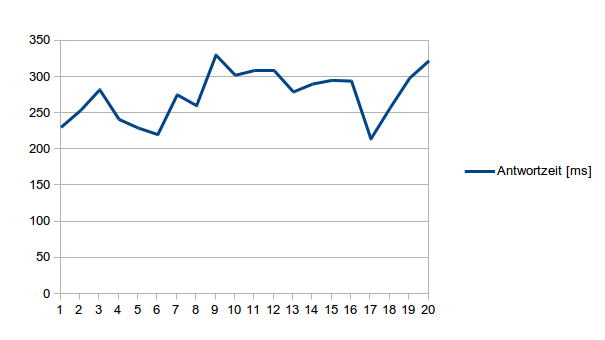
\includegraphics[width=150mm]{images/ch6_img01_response_time.png}
\caption{Antwortzeit der GameAPI für den Tag public\_transport=stop\_area}
\label{img:ch6_img01_response_time}
\end{center}
\end{figure}

Abweichungen der Antwortzeit sind weniger bedeutend, da das Spielfeld sich bereits vorher für den Spieler aufbaut und die Spielelemente mittels Ajax Request geladen werden. Darüber hinaus wird durch die dynamische Erweiterung der Bounding Box sichergestellt, dass alle Elemente am Rand der Karte bereits geladen sind. Das Nachladen der Elemente beim Fortbewegen kann daher auch minimal länger dauern, da das Spielfeld immer zentriert auf den Spieler ist.

Durch die Kapselung der einzelnen Module wird auch sichergestellt, dass eine Erweiterbarkeit der Spielmechnaik ohne größeren Aufwand möglich ist. Das entsprechende Beispielspiel kann problemlos erweitert werden oder aber durch ein beliebiges anderes Spiel ersetzt werden.
Hierbei zeigt sich, dass die Anforderung für die Flexibilität des Frameworks hinsichtlich seiner Erweiterbarkeit und Austauschbarkeit gegeben ist.

\subsection*{Relokalisierbarkeit}

Der nächste essentielle Aspekt der Problemstellung war die Relokalisierbarkeit. Ziel war es im Zuge des einfachen Stagings dem Spielleiter entsprechend eine Möglichkeit an die Hand zu geben, welche im auch ein Spielen außerhalb eines festen Bereiches ermöglicht. Hierzu wurden entsprechende OSM-Daten verwendet die durch eine Transformation zu Spielelementen umgewandelt wurden. Durch die entsprechende Evaluation der OSM Tags im Voraus wird sichergestellt, dass der jeweilige beste Tag für die getesteten Umgebungen ausgewählt wurde. 

-Verarbeitung von Geodaten
-Einbindung der lokalen Händlern

\subsection*{Verwendbarkeit von OSM Daten}
-OSM-Daten Transformation/Aufbereitung

-vergleich zu den anforderungen


Für den Spielleiter lässt sich daher festhalten, dass die Anforderung für ein einfaches Staging erfüllt wird. Darüberhinaus findet auch die geforderte Modularisierung der einzelnene Funktionen statt.

Was ist noch zu tun?

\section{Qualität der Spielfelder}
\label{ch:CH6_qualtiy_of_gameboards}

